\chapter{Retro-fallback}
\label{chapter:rfb}

\ifpdf
    \graphicspath{{chapter0x-rfb/}}
\else
    \graphicspath{}
\fi

This chapter presents a novel retrosynthesis algorithm called \emph{retro-fallback}.
Unlike previous algorithms,
retro-fallback is designed to account for uncertainty about synthesis plans.
The content of this chapter was recently published as a
conference paper in ICLR 2024 \citep{tripp2023retrofallback}.
The paper was jointly written with
my supervisor José Miguel Hernández-Lobato
and collaborators
Krzysztof Maziarz, Sarah Lewis, and Marwin Segler
from Microsoft Research Cambridge.
I was the lead contributor to the project,
but all authors contributed to the writing of the manuscript.

\section{Motivation}
\label{sec:rfb:motivation}

As explained in detail in \S\ref{sec:background:synthesis},
retrosynthesis is important to characterize the space of available molecules
$\amolspace$ for molecule optimisation problems.
Although machine learning has recently enabled a lot of progress in retrosynthesis algorithms
\citep{strieth2020machine,tu2023predictive,stanley2023fake},
there are still barriers to translating the output of retrosynthesis algorithms into real-world syntheses.
One significant issue is that these algorithms have imperfect knowledge of the space of chemical reactions.
Because the underlying physics of chemical reactions cannot be efficiently simulated,
retrosynthesis algorithms typically rely on data-driven reaction prediction models which can ``hallucinate'' unrealistic
or otherwise infeasible reactions~\citep{zhong2023retrosynthesis}.
This results in synthesis plans which cannot actually be executed.

Although future advances in modelling may reduce the prevalence of infeasible reactions,
we think it is unlikely that they will ever be eliminated entirely, as even the plans of expert chemists do not always work on the first try.
One possible workaround to failing plans is to produce \emph{multiple} synthesis plans instead of just a single one:
the other plans can act as \emph{backup} plans in case the primary plan fails.
Although existing algorithms may find multiple synthesis plans, they are generally not designed to do so,
and there is no reason to expect the plans found will be suitable as \emph{backup} plans (e.g.\@ they may share steps with the primary plan and thereby also share the same failure points).

In this chapter, we present several advancements towards retrosynthesis with backup plans.
First, in section~\ref{sec:retrosynthesis formalism} we explain how uncertainty about whether a synthesis plan will work in the lab
can be quantified with stochastic processes.
We then propose an evaluation metric called \emph{successful synthesis probability} (SSP) which quantifies the probability that \emph{at least one}
synthesis plan found by an algorithm will work. This naturally captures the idea of producing backup plans.
Next, in section~\ref{sec:retro fallback} we present a novel search algorithm called \emph{retro-fallback}
which greedily optimises SSP.
Finally, in section~\ref{sec:rfb:experiments} we demonstrate quantitatively that retro-fallback outperforms existing algorithms on several \textit{in-silico} benchmarks.
Together, we believe these contributions form a notable advancement towards translating results from retrosynthesis algorithms into the lab.

\section{Reformulating retrosynthesis with uncertainty}\label{sec:retrosynthesis formalism}

The ``standard'' formulation of retrosynthesis presented in
\S\ref{sec:background:synthesis} requires knowledge of which reactions are possible
(encoded by the backward reaction model $B$)
and which molecules are purchasable (encoded by the inventory $\gI$).
In reality, neither of these things are perfectly known.
As mentioned in the introduction,
predicting the outcome of chemical reactions is difficult even for experts,
and machine learning models for $B$ can ``hallucinate'' unrealistic reactions.
Perhaps surprisingly, it is also not totally clear which molecules can be bought.
Things like shipping delays mean you might not always receive molecules which you order.
However, many companies now advertise large ``virtual libraries'' with billions of molecules
which they \emph{believe} they can synthesize upon request, but not with 100\% reliability.\footnote{ For example, \href{https://enamine.net/}{Enamine} a popular supplier, only claims that \href{https://enamine.net/compound-collections/real-compounds}{80\% of its virtual ``REAL'' library can be made}.}
This section presents our first main contribution to account for this:  %
a novel formulation of retrosynthesis which explicitly represents uncertainty.

\subsection{Stochastic processes for ``feasibility'' and ``buyability''}

There are many reasons why chemists may consider a reaction unsuccessful,
ranging from having a low yield to producing the wrong product altogether.
Similarly, ``unsuccessfully'' buying a molecule
could indicate anything from a prohibitively high cost to the molecule not being delivered.
In either case, for simplicity we propose to collapse this nuance into a binary outcome:
reactions are either \emph{feasible} or \emph{infeasible},
and molecules are either \emph{buyable} or not.
We therefore postulate the existence of an unknown
``feasibility'' function $f^*:\gR\mapsto\{0,1\}$
and ``buyability'' function $b^*:\gM\mapsto\{0,1\}$.

Uncertainty about $f^*$ and $b^*$ can be represented
by \emph{stochastic processes} (essentially distributions over functions).
We define a \emph{feasibility model} $\xi_f$ to be a binary stochastic process over $\gR$,
and define a \emph{buyability model} $\xi_b$ to be a binary stochastic process over $\gM$.
This formulation is very general:
$\xi_f$ and $\xi_b$ not only represent beliefs
of $\probability\left[f^*(r)=1\right]$
and $\probability\left[b^*(m)=1\right]$
for all molecules $m$ and reactions $r$,
but also allows \emph{correlations} between feasibilities and buyabilities to be modelled.

Although this formalism may seem esoteric,
it is possible to re-cast almost all existing approaches to reaction prediction
as stochastic processes.
Any model which implicitly assigns a probability
to each reaction (e.g.\@ the softmax outputs of a neural network)
can be trivially converted into a stochastic process by assuming that all outcomes are independent.
Correlations can be induced via Bayesian inference over the model's parameters
\citep{mackay1992practical}
or using a non-parametric model like a Gaussian process
\citep{rasmussen2006gp}.
Importantly however,
it is not at all clear how to produce \emph{realistic}
models $\xi_f$  and $\xi_b$.
Intuitively,  producing such models is at least as challenging
as predicting reaction outcomes \emph{without} uncertainty estimates,
which is itself an active (and challenging) research area.
Therefore, we will generally discuss $\xi_f$/$\xi_b$ in a model-agnostic way. %

\subsection{New evaluation metric: successful synthesis probability (SSP)}

Given $f$ and $b$,
a synthesis plan $T$ is \emph{successful} if all its reactions $r$ are feasible ($f(r)=1$)
and all its starting molecules $m$ are buyable ($b(m)=1$).
We formalize this with the function
\begin{equation}\label{eqn:success defn for single synthesis plan}
    \sigma(T;f,b) = \begin{cases}
        1 & f(r)=1\ \forall r\in T,\ b(m)=1\text{ and } \forall m\in\frontier(T) \\
        0 & \text{otherwise}
    \end{cases}\ .
\end{equation}
Finding successful synthesis plans is a natural goal of retrosynthesis.
Of course, because $f$ and $b$ are unknown, 
we can at best search for synthesis plans with a high \emph{probability}
of being successful.
Given a \emph{set} of synthesis plans $\mathcal{T}$,
we define the \emph{successful synthesis probability} (SSP) as:
\begin{equation}\label{eqn:SSP defn}
    \mathrm{SSP}(\mathcal T ; \xi_f, \xi_b) =
    \probability_{f\sim\xi_f, b\sim\xi_b}\left[
        \exists\ T\in\mathcal T\text{ with } 
        \sigma(T;f,b)=1
    \right]
\end{equation}
Given just a single plan $T$,
$\mathrm{SSP}(\{T\};\xi_f,\xi_b)=\mathbb E_{f,b}\left[\sigma(T;f,b)\right]$
and represents the probability that $T$ is successful,
which we will hereafter refer to as the \emph{success probability} of $T$.
When $\mathcal T$ contains multiple synthesis plans, then 
SSP quantifies the probability that \emph{any} of these synthesis plans is successful.
We argue that SSP is a good evaluation metric for the
synthesis plans produced by retrosynthesis
search algorithms.
It simultaneously captures the goals of 
producing synthesis plans with high success probability
and producing ``backup'' plans
which could succeed if the primary synthesis plan does not.
Note that by definition, SSP is non-decreasing with respect to $\mathcal T$,
implying that an algorithm will never be penalized for producing additional synthesis plans.


\subsection{
    Efficiently estimating SSP for all synthesis plans in 
    \texorpdfstring{$\enumplans_{\targetmol}(\gG')$}{P(G)}
}

Recall from \S\ref{sec:background:synthesis} that many retrosynthesis search algorithms
do not directly output synthesis plans:
they produce a search graph $\gG'$ which (implicitly)
contains a set of synthesis plans $\enumplans_{\targetmol}(\gG')$.
Therefore, it is natural to calculate the SSP of the entire set $\enumplans_{\targetmol}(\gG')$.
However, this set may be combinatorially large,
making calculating SSP by enumerating $\enumplans_{\targetmol}(\gG')$ intractable.
Instead, we propose a method to estimate SSP using functions sampled from $\xi_f$ and $\xi_b$.

Let 
$\rs(n; \gG',f,b):\gM\cup\gR\mapsto\{0,1\}$
define the \emph{success} of a node $n\in\gG$:
whether \emph{any} successful synthesis plan in $\gG$ contains $n$
(we write $\rs(n)$ when $\gG',f,b$ are clear from context).
$\rs(n)$ will satisfy
\begin{equation}\label{eqn:s and sigma relationship}
    \rs(n;\gG',f,b)
    \stackrel{\text{(A)}}{=}
    \sigma(T^*;f,b)
    \stackrel{\text{(B)}}{=}
    \rs(n;T^*,f,b)
    ,\qquad
    T^*\in\argmax_{
        T\in\enumplans_{*}(\gG'):\ n\in T
    }
        \sigma(T;f,b)\ ,
\end{equation}
where $\enumplans_{*}(\gG')=\bigcup_{m\in\gG'}\enumplans_m(\gG')$ is the set of all synthesis plans for all molecules in $\gG'$.
Equality (A) follows directly from the definition above,
and equality (B) holds because $T^*$
would still satisfy the $\arg\max$ if nodes not in $T^*$ were pruned from $\gG'$.
Let $\children_{\gG'}(n)$ denote the children of node $n$.
For a reaction $r\in\gG'$ to succeed,
it must be feasible ($f(r)=1$) and have all its reactant molecules
$m'\in\children_{\gG'}(r)$ succeed.
Conversely, a molecule $m\in\gG'$ will succeed
if it is buyable ($b(m)=1$) or if any reaction producing $m$ succeeds.
This suggests $\rs(\cdot)$ will satisfy the recursive equations
\begin{align}
    \rs(m;\gG',f,b) &= 
        \max\left[
            b(m),
            \max_{r\in\children_{\gG'}(m)}\rs(r;\gG',f,b)
        \right]\ , \label{eqn:molecule success}\\
    \rs(r;\gG',f,b) &=
        f(r) \prod_{m\in\children_{\gG'}(r)} \rs(m;\gG',f,b)
    \ . \label{eqn:reaction success}
\end{align}
SSP can then be estimated by averaging $\rs(\targetmol)$
over $k$ i.i.d.\@ functions sampled from $\xi_f$ and $\xi_b$:
\begin{equation}\label{eqn:estimating SSP from s}
    \mathrm{SSP}(\enumplans_{\targetmol}(\gG') ; \xi_f, \xi_b)
    \stackrel{\text{(A)}}{=}
    \probability_{f\sim\xi_f, b\sim\xi_b}\left[
        \rs(\targetmol;\gG',f,b) = 1
    \right]
    \approx
    \frac{1}{k}\sum_{i=1}^k
        \rs(\targetmol;\gG',f_k,b_k)
    \ .
\end{equation}
Note that equality (A) above follows directly from
equations~\ref{eqn:SSP defn} and \ref{eqn:s and sigma relationship}.
The existence of such recursive equations suggests that $\rs(\cdot)$
could be efficiently computed for all nodes in $\gG'$ in polynomial time
using dynamic programming
(we discuss this further in Appendix~\ref{appendix:proofs:polynomial-dp-updates}),
allowing an overall polynomial time estimate of SSP.
That being said, it is still only an \emph{estimate}.
Unfortunately, we are able to prove that an exact calculation is generally intractable.
\begin{theorem}\label{thm:success prob is NP hard}
    Unless $P=NP$, there does not exist an algorithm to compute 
    \begin{equation*}
        \mathrm{SSP}(\enumplans_{\targetmol}(\gG') ; \xi_f, \xi_b)  
    \end{equation*}
    for arbitrary
    $\xi_f,\xi_b$ whose time complexity grows polynomially with the number of nodes
    in $\gG'$.
\end{theorem}
The proof is given in Appendix~\ref{appendix:proofs:succ-prob-np-hard}.
We therefore conclude that estimating SSP using equation~\ref{eqn:estimating SSP from s}
is the best realistic option given limited computational resources.

\section{Retro-fallback: a greedy algorithm to maximise SSP}\label{sec:retro fallback}


\subsection{Ingredients for an informed, greedy search algorithm}\label{sec:retro fallback ingredients}

Intuitively, a greedy search algorithm would expand molecules in $\frontier(\gG')$
which are predicted to improve SSP.
Given that calculating SSP exactly is intractable,
calculating potential changes is likely to be intractable as well.
Therefore, we will estimate SSP changes by averaging over samples 
from $\xi_f$ and $\xi_b$,
and will consider how expansion might change $\rs(\targetmol;\gG',f,b)$
for fixed  samples $f,b$.

Specifically, we consider the effect of simultaneously expanding \emph{every} frontier
molecule on a fixed synthesis plan $T\in\enumplans_{*}(\gG')$.\footnote{
    We do not consider expanding just a single node because,
    for a reaction with multiple non-buyable reactant molecules in $\frontier(\gG')$,
    expanding just \emph{one} reactant will never produce a new successful synthesis plan.
}
We represent the hypothetical effect of such an expansion
with a random function $e_{T}:\gM\mapsto\{0,1\}$,
where $e_{T}(m)=1$ implies that expanding $m$ produces a new successful synthesis plan for $m$.
We assume the value of $e_{T}$ is independently distributed for every molecule,
with probabilities given by
a \emph{search heuristic} function
$h:\gM\mapsto[0,1]$
\begin{equation}\label{eqn:eT expansion function}
    \probability_{e_{T}}\left[e_{T}(m)=1\right] =
    \begin{cases}
        h(m) & m\in\frontier(\gG')\cap {T} \\
        0 & m\notin\frontier(\gG')\cap {T}
    \end{cases} \ .
\end{equation}

The effect of this expansion on the success of $T$ is given by
$\sigma':\enumplans_*(\gG')\mapsto\{0,1\}$,
defined as
\begin{equation}\label{eqn:expansion success single plan}
    {\color{blue} \sigma '} (T;f,b,{\color{blue}e_{T}}) =
    \begin{cases}
        1 & f(r)=1\ \forall r\in T\text{ and } \left(b(m)=1{\color{blue}\text{ or } e_{T}(m)=1}\right) \forall m\in\frontier(T) \\
        0 & \text{otherwise}
    \end{cases}\ .
\end{equation}

Equation~\ref{eqn:expansion success single plan} for $\sigma'$
is almost identical to equation~\ref{eqn:success defn for single synthesis plan} for $\sigma$.
The key difference (\textcolor{blue}{highlighted})
is that $T$ can be successful if a starting molecule $m$ is not buyable ($b(m)=0$)
but has instead had $e_{T}(m)=1$.
Recalling that $e_{T}$ is a random function,
we define
$\bar\sigma':\enumplans_*(\gG')\mapsto[0,1]$ as
\begin{equation}\label{eqn:sigma' bar}
    \bar\sigma'(T;f,b,h) =
    \mathbb E_{e_{T}} \left[
        \sigma'(T;f,b, e_{T}
    \right]\ ,
\end{equation}
namely the \emph{probability} that a synthesis plan $T$ will be successful upon expansion.%
\footnote{
    The dependence on $h$ is because it
    defines the distribution of $e_{T}$ in equation~\ref{eqn:expansion success single plan}.
}
A natural choice for a greedy algorithm could be to expand
frontier nodes on synthesis plans $T$ with high $\bar\sigma'(T;f,b,h)$.
However, not all synthesis plans contain frontier nodes
(e.g.\@ plan $T_1$ in Figure~\ref{fig:retrosynthesis-background-schematic}b)
or produce $\targetmol$.
To select frontier nodes for expansion,
we define the function $\tilde\rho:\gM\cup\gR\mapsto[0,1]$ by
\begin{equation}\label{eqn:rho tilde}
    \tilde\rho(n;\gG',f,b,h) = \max_{T\in\enumplans_{\targetmol}(\gG'):\ n\in T}
        \bar\sigma'(T;f,b,h)\ ,\qquad n\in\gG'\ .
\end{equation}
For $m\in\frontier(\gG')$,
$\tilde\rho(m)$ represents the highest estimated success probability
of all synthesis plans for $\targetmol$ which also contain $m$
(conditioned on a particular $f,b$).
Therefore, a greedy algorithm could sensibly expand frontier molecules $m$ with maximal $\tilde\rho(m)$.

Unfortunately, the combinatorially large number of synthesis plans
in a graph $\gG'$ makes evaluating $\tilde\rho$ potentially infeasible.
To circumvent this,
we assume that no synthesis plan in $\gG'$ uses the same molecule in
two separate reactions, making all synthesis plans trees
(we will revisit this assumption later).
This assumption guarantees that the outcomes from different branches
of a synthesis plan will always be independent.
Then, to help efficiently compute $\tilde\rho$,
we will define the function
\begin{equation}\label{eqn:psi tilde}
    \tilde\psi(n;\gG',f,b,h)=\max_{T\in\enumplans_*(\gG'):\ n\in T}\bar\sigma'(T;f,b,h)
\end{equation}
for every node $n\in\gG'$.
$\tilde\psi$ is essentially a less constrained version of $\tilde\rho$.
The key difference in their definitions is that $\tilde\psi$
maximises over \emph{all} synthesis plans containing $n$,
including plans which do not produce $\targetmol$.
The independence assumption above
means that 
$\tilde\psi$ has a recursively-defined analytic solution
$\psi(\cdot;\gG',f,b,h):\gM\cup\gR\mapsto[0,1]$
given by the equations
\begin{align}
    \psi(m;\gG',f,b,h) &= \begin{cases}
    \max\left[b(m), h(m)\right] & m\in\frontier(\gG') \\
    \max\left[b(m), \max_{r\in\children_{\gG'}(m)}\psi(r;\gG',f,b,h) \right] & m\notin\frontier(\gG') \\
    \end{cases} \ ,\label{eqn:psi molecule} \\
    \psi(r;\gG',f,b,h) &= f(r) \prod_{m\in\children_{\gG'}(r)} \psi(m;\gG',f,b,h)\ . \label{eqn:psi reaction}
\end{align}
Details of this solution are presented in Appendix~\ref{appendix:rfbd:s,psi,rho}.
$\psi(n)$ can be roughly interpreted as ``the best expected success value for $n$ upon expansion.''
In fact,
the relationship between $\psi$ and $\bar\sigma'$ is exactly analogous
to the relationship between $\rs$ and $\sigma$ in equation~\ref{eqn:s and sigma relationship}.

To compute $\tilde\rho$, first note that $\tilde\rho(\targetmol)=\tilde\psi(\targetmol)$,
as for $\targetmol$ the constraints in equations~\ref{eqn:rho tilde}
and \ref{eqn:psi tilde} are equivalent.
Second, because of the independence assumption above,
the best synthesis plan containing \emph{both} a node $n$ and its parent $n'$
can be created by taking an optimal synthesis plan for $n'$ (which may or may not contain $n$),
removing the part ``below'' $n'$, and adding in an (unconstrained) optimal plan for $n$.
Letting $\parents_{\gG'}(\cdot)$ denote a node's parents,%
\footnote{
    Recall that because we 
    consider only single-product reactions,
    all reaction nodes will have exactly one parent,
    making equation~\ref{eqn:rho reaction} well-defined.
}
under this assumption $\tilde\rho$
has a recursively-defined analytic solution
$\rho(\cdot;\gG',f,b,h):\gM\cup\gR\mapsto[0,1]$ defined as
\begin{align}
     \rho(m;\gG',f,b,h) &= \begin{cases}
    \psi(m;\gG',f,b,h) & m\text{ is target molecule }\targetmol \\
    \max_{r\in\parents_{\gG'}(m)}\rho(r;\gG',f,b,h) & \text{all other }m \\
    \end{cases}\ , \label{eqn:rho molecule} \\
    \rho(r;\gG',f,b,h) &= \begin{cases}
        0 & \psi(r;\gG',f,b,h) = 0 \\
        \rho(m';\gG',f,b,h) \frac{\psi(r;\gG',f,b,h)}{\psi(m';\gG',f,b,h)} & \psi(r;\gG',f,b,h) > 0, m'\in\parents_{\gG'}(r)
    \end{cases}\ .
    \label{eqn:rho reaction}
\end{align}
Details of this solution are presented in Appendix~\ref{appendix:rfbd:s,psi,rho}.
Like $\rs(\cdot)$,
$\psi$ and $\rho$ have recursive definitions,
and can therefore be calculated with dynamic programming techniques.
Since $\psi$ depends on a node's children, it can generally be calculated
``bottom-up'',
while $\rho$ can be calculated ``top-down'' because it depends on a node's parents.
We discuss details of computing $\psi$ and $\rho$ in Appendix~\ref{appendix:rfbd:s,psi,rho}.


However, in deriving $\psi$ and $\rho$
we assumed that all synthesis plans
$T\in\enumplans_{*}(\gG')$ were trees.
In practice, this assumption may not hold.
If this assumption is violated,
$\psi$ and $\rho$ can both still be calculated,
but will effectively \emph{double-count} molecules which occur multiple times in a synthesis plan,
and therefore not equal $\tilde\psi$ and $\tilde\rho$.
This is a well-known issue in AND/OR graphs:
for example,
\citet[page 102]{nilsson1982principles}
describes the essentially same issue when calculating minimum cost synthesis plans.
Ultimately we will simply accept this and use 
$\psi$/$\rho$ instead of
$\tilde\psi$/$\tilde\rho$
despite their less principled interpretation,
chiefly because the recursive definitions of $\psi$/$\rho$ are amenable to efficient computation.
Synthesis plans which use the same molecule twice
are unusual in chemistry;
therefore we do not expect this substitution to be problematic in practice.


\subsection{Retro-fallback: a full greedy algorithm}
\label{ssec:retro-fallback algorithm}

Recall our original goal at the start of section~\ref{sec:retro fallback ingredients}:
to estimate how expansion might affect SSP.
We considered \emph{a single sample} $f\sim\xi_f$ and $b\sim\xi_b$,
and developed the function $\rho$,
which for each frontier
molecule $m\in\frontier(\gG')$ gives the best estimated synthesis plan for $\targetmol$
if $m$ is expanded
(simultaneously along with other frontier molecules on an optimally chosen synthesis plan).
We will now use $\rho$ to construct a full algorithm.

Expanding a frontier molecule can improve SSP if, for samples $f$ and $b$
where \\ $\rs(\targetmol;\gG',f,b)=0$,
the expansion changes this to 1.
In this scenario, expanding a frontier molecule
$m^*\in\argmax_{m\in\frontier(\gG')}\rho(m;\gG',f,b,h)$
is a prudent choice,
as it lies on a synthesis plan with the highest probability
of ``flipping'' $\rs(\targetmol;\gG',f,b)$ to $1$.
In contrast, because $\rs(\cdot)$ will never decrease as nodes are added,
if $\rs(\targetmol;\gG',f,b)=1$ then it does not matter which molecule is expanded.
Therefore, when aggregating over samples of $f$ and $b$ to decide which molecules to expand to improve SSP,
we will consider the value of $\rho$ \emph{only} in cases when $\rs(\targetmol;\gG',f,b)=0$.


For our greedy algorithm,
we propose to simply expand the molecule with the highest \emph{expected improvement}
of SSP.
Letting $\1_{(\cdot)}$ be the indicator function,
this is a molecule
$m\in\frontier(\gG')$ which maximises
\begin{equation}\label{eqn:retro fallback alpha}
    \alpha(m;\gG',\xi_f,\xi_b, h) = \E_{f\sim \xi_f, b\sim \xi_b}\left[
        \1_{\rs(\targetmol;\gG',f,b)=0}\left[\rho(m;\gG',f,b,h)\right]
    \right]
\end{equation}
In practice, $\alpha$ would be estimated from a finite number of samples from $\xi_f$ and $\xi_b$.
Using $\rho$ to select a \emph{single} molecule may seem odd,
especially because $\rho$ is defined as a hypothetical outcome of simultaneously expanding multiple nodes.
However, note that in principle there is nothing problematic about expanding these nodes one at a time.

We call our entire algorithm \emph{retro-fallback} (from ``retrosynthesis with fallback plans'')
and state it explicitly in Algorithm~\ref{alg:retro-fallback-full}.
The sections are colour-coded for clarity.
After initializing $\gG'$, the algorithm performs
$L$ iterations of expansion
(although this termination condition could be changed as needed).
In each iteration, first \textcolor{blue}{the values of $\rs$, $\psi$, and $\rho$ are computed for each sample of $f$ and $b$}.\footnote{
This order is chosen because $\rs$ depends only on $f$ \& $b$, $\psi$ depends on $\rs$, and $\rho$ depends on $\psi$.
Because the optimal algorithm to compute $\rs,\psi,\rho$ may depend on $\gG'$,
we only specify this computation generically.
}
Next, \textcolor{orange}{the algorithm checks whether there are no frontier nodes or whether the estimated SSP is 100\%, and if so terminates}
(both of these conditions mean no further improvement is possible).
Finally, \textcolor{violet}{a frontier node maximising $\alpha$ (\ref{eqn:retro fallback alpha}) is selected and expanded}.
Of course, a practical implementation of retro-fallback may look slightly different from Algorithm~\ref{alg:retro-fallback-full},
using techniques such as caching and vectorized operations to improve efficiency.

\begin{algorithm}[tb]
\caption{Retro-fallback algorithm (see~\ref{ssec:retro-fallback algorithm})}\label{alg:retro-fallback-full}
\begin{algorithmic}[1]
\REQUIRE target molecule $\targetmol$, max iterations $L$, backward reaction model $B$, search heuristic $h$
\REQUIRE samples $f_1,\ldots,f_k\sim\xi_f$, $b_1,\ldots,b_k\sim\xi_b$
\STATE $\gG'\gets \{\targetmol\}$
\FOR{$i$ in $1,\ldots,L$}
    {
    \color{blue} 
    \FOR{$j$ in $1,\ldots,k$}
        \STATE Compute $\rs(\cdot;\gG',f_j,b_j)$ for all nodes using equations~\ref{eqn:molecule success}--\ref{eqn:reaction success}
        \STATE Compute $\psi(\cdot;\gG',f_j,b_j,h)$ for all nodes using equations~\ref{eqn:psi molecule}--\ref{eqn:psi reaction}
        \STATE Compute $\rho(\cdot;\gG',f_j,b_j,h)$ for all nodes using equations~\ref{eqn:rho molecule}--\ref{eqn:rho reaction}
    \ENDFOR
    }

    {\color{orange}
    \STATE\label{early termination} Terminate early if $|\frontier(\gG')|=0$ OR $\rs(\targetmol;\gG',f_j,b_j)=1 \,\forall j$}

    {\color{violet}
    \STATE $m_{(i)}\gets \arg\max_{m\in \frontier(\gG')}\alpha(m;\gG',\xi_f,\xi_b, h)$ (equation~\ref{eqn:retro fallback alpha}, breaking ties arbitrarily) 
    \STATE Add all reactions and molecules from $B(m_{(i)})$ to $\gG'$
    }
\ENDFOR
    
\RETURN $\gG'$
\end{algorithmic}
\end{algorithm}






\section{Related Work}

Retro-fallback is most comparable with other retrosynthesis
search algorithms including
MCTS \citep{segler2018planning},
retro* \citep{chen2020retro},
and proof number search \citep{heifets2012construction,kishimoto2019depth}.
As mentioned in \S\ref{sec:background:synthesis},
at a high level these algorithms are all similar:
they use a heuristic to guide the construction of an explicit search graph.
However, previous algorithms may struggle to maximise SSP
because their internal objectives consider only \emph{individual} synthesis plans,
while SSP depends on \emph{multiple} synthesis plans simultaneously.
For most algorithms, the best proxy for SSP is likely to maximise the success probability of individual synthesis plans:
an objective which may not always perfectly align with maximising SSP.%
\footnote{
    For example, finding many plans with high success probability but are highly correlated
    may not maximise SSP.
}
In contrast, retro-fallback is specifically designed to maximise SSP.

Mechanistically, retro-fallback most closely resembles retro* \citep{chen2020retro},
which was introduced in more detail in \S\ref{sec:background:retro*}.
Both retro* and retro-fallback
perform a bottom-up and top-down update
to determine the value of each potential action, then select actions greedily.
In fact, $\psi$ and $\rho$ have cost-minimisation interpretations
(see Appendix~\ref{appendix:s,psi,rho min cost}).
The key difference between retro* and retro-fallback is the node selection step:
retro* considers just a single cost for each node,
while retro-fallback aggregates over a vector of samples
to directly optimise SSP.

Lastly, we note that 
prior works have also considered planning in stochastic graphs,
albeit in other contexts.
For example, the ``Canadian Traveller Problem'' and its variants \citep{papadimitriou1991shortest}
study search on a graph where edges can be randomly deleted.%
\footnote{
    The original problem statement was to find a path between two cities in Canada,
    where roads may be randomly blocked by snow and force the driver to turn back
    and find an alternative path
    (in reality however, Canadians simply drive through the snow).
}
However, this is an \emph{online} problem,
meaning that the planning algorithm learns about edge deletions during the planning process.
In contrast, our algorithm assumes \emph{offline} planning
because chemists desire complete synthesis plans \emph{before} performing any lab experiments.
Moreover, works in this area seem to assume explicit OR graphs with independent probabilities,
while our problem uses implicit AND/OR graphs with non-independent probabilities.

\section{Experiments}\label{sec:rfb:experiments}

In this section we evaluate retro-fallback experimentally.
The key question we seek to answer is whether retro-fallback does indeed maximise SSP
more effectively than existing algorithms.
We built our code around the open-source library \textsc{syntheseus}
\citep{maziarz2023re}.\footnote{
    https://github.com/microsoft/syntheseus/
}
Code to reproduce the experiments is available at \retrofallbackcodeurl{}.

\subsection{Experiment Setup}

We have based our experiment design on the USPTO benchmark from \citet{chen2020retro},
which has been widely used to evaluate multi-step retrosynthesis algorithms.
However, because this benchmark does not include a feasibility or buyability model
we have made some adaptations to make it suitable for our problem setting.
Importantly, because we do not know what the ``best'' feasibility model is, we instead
test \emph{multiple} feasibility models in the hope that the conclusions of our experiments
could potentially generalize to future, more advanced feasibility models.

We base all of our feasibility models on the pre-trained template classifier from \citet{chen2020retro}
restricted to the top-50 templates.
We vary our feasibility model across two axes: the \emph{marginal} feasibility assigned to each reaction
and the \emph{correlation} between feasibility outcomes.
Marginally, we consider a constant value of $0.5$,
and a value which starts at $0.75$ and decreases with the rank of the reaction
in the template classifier's output, given by
\begin{equation}
    p(\mathrm{rank}) = \frac{0.75}{\mathrm{rank}/10}\ .
\end{equation}
For correlations, we consider all outcomes being independent or determined by a latent GP model
defined by the equations
\begin{align}
    \mathrm{outcome}(z) &= \1_{z > 0} \\
    z(r) &\sim \mathcal{GP}\left(\mu(\cdot), K(\cdot, \cdot)\right) \\
    \mu(r) &= \Phi^{-1}\left(\probability[f(r)=1]\right) \\
    K(r,r) &= 1 \quad\forall r \ .    \label{eqn:gplvm:variance} 
\end{align}
Here, $\Phi$ represents the CDF of the standard normal distribution.
Because of equation~\ref{eqn:gplvm:variance},
the marginal distribution of each reaction's $z$ value is $\mathcal{N}(\Phi^{-1}(p(r)), 1)$
which will be positive with probability $\probability[f(r)=1]$
(i.e.\@ it preserves arbitrary marginal distributions).
If $K$ is the identity kernel (i.e.\@ $K(r_1,r_2)=\1_{r_1=r_2}$) then this model implies all outcomes are independent.
However, non-zero off-diagonal values of $K$ will induce correlations (positive or negative).

We aimed to design a model which assigns correlations very conservatively:
only reactions involving similar molecules \emph{and} which induce similar changes in the reactant molecules
will be given a high positive correlation; all other correlations will be near zero.
We therefore chose a kernel as a product of two simpler kernels:
\begin{equation*}
    K_\text{total}(r_1,r_2)=K_\text{mol}(r_1,r_2)K_\text{mech}(r_1,r_2)\ .
\end{equation*}
We chose $K_\text{mol}(r_1,r_2)$ to be the Tanimoto kernel
$T_{MM}$ from chapter~\ref{chapter:trf} (equation~\ref{eqn:minmax-kernel})
between the count Morgan fingerprints (defined \S\ref{definition:morgan-fingerprint})
with radius 1 of the entire set of product and reactant molecules.\footnote{
This is the same as adding the fingerprint vectors for all component molecules.
}
We chose $K_\text{mech}(r_1,r_2)$ to be $T_{MM}$ on the \emph{difference} vectors between the product and reactant fingerprints individually.
The difference vector between two molecular fingerprints will essentially yield the set of subgraphs
which are added/removed as part of the reaction.
For this reason, it has been used to create representations of chemical reactions
in previous work \citep{schneider2015development}.

Analogous to \citet{chen2020retro},
we create a buyability model based on the \href{https://www.emolecules.com/}{eMolecules} library
which designates only chemicals shipped within 10 business
days
as 100\% buyable.

We compare retro-fallback to breadth-first search (an uninformed search algorithm)
and the heuristic-guided algorithms retro* \citep{chen2020retro} and MCTS \citep{segler2018planning, genheden2020aizynthfinder, coley2019robotic}.
All algorithms were implemented
using the \textsc{syntheseus} library \citep{maziarz2023re}
and run with a fixed budget of calls to $B$.
Retro-fallback was run with $k=256$ samples from $\xi_f,\xi_b$.
MCTS and retro* were configured to maximise SSP by 
replacing costs or rewards from the backward reaction model $B$
with quantities derived from $\xi_f$ and $\xi_b$.
In particular, retro* was configured to use the reaction cost 
$-\log{\E_f[f(r)]}$,
and MCTS used an estimate of $\sigma(T;\xi_f,\xi_b)$ as its reward function.
However,
the presence of heuristics makes comparing algorithms difficult.
Because the choice of heuristic will strongly influence an algorithm's behaviour,
we tried to use similar heuristics for all algorithms
to ensure a meaningful comparison.
Specifically,
we tested an \emph{optimistic} heuristic
(which gives the best possible value for each frontier node)
and a heuristic based on the synthetic accessibility (SA) score \citep{ertl2009estimation},
which has been shown to be a good heuristic for retrosynthesis in practice
despite its simplicity \citep{skoraczynski2023critical}.
For retro-fallback, this heuristic was
\begin{equation*}
    h_\text{SA}(m) = 1 - \frac{\mathrm{SA}(m)-1}{10}\ .
\end{equation*}
The SA score heuristic was minimally adapted for each algorithm
to roughly have the same interpretation:
in particular, taking the negative logarithm for retro*
and multiplying the heuristic for all molecules in a state for MCTS.

We tested all algorithms on the set of 190 ``hard''
molecules from \citet{chen2020retro},
which do not have straightforward synthesis plans.
We also tested on a set of 1000 molecules chosen from the
GuacaMol test set \citep{brown2019guacamol}.
Our primary evaluation metric is the SSP values estimated with $k=10\,000$ samples,
averaged over all test molecules.

\subsection{How effective is retro-fallback at maximising SSP?}\label{sec:experiment:how effective is retro fallback}

\begin{figure}
    \centering
    {\large SA score heuristic} \\
    \vspace{0.3cm}
    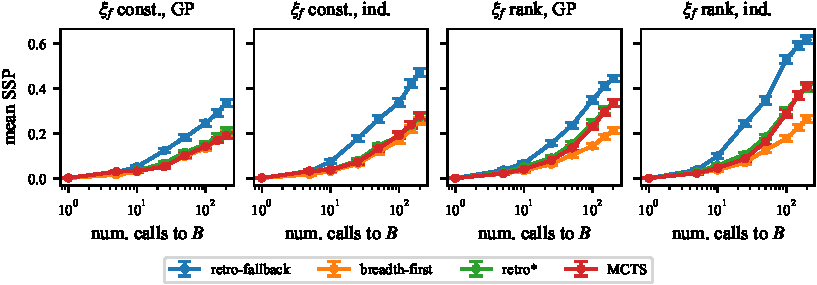
\includegraphics{figures/comparison/retrostar190/ssp_sascore.pdf}
    \vspace{0.3cm}
    {\large optimistic heuristic} \\
    \vspace{0.3cm}
    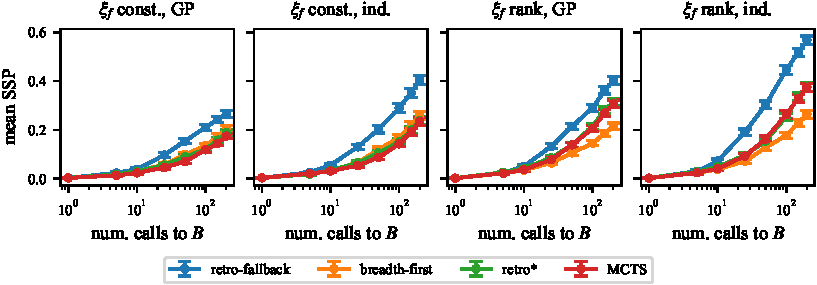
\includegraphics{figures/comparison/retrostar190/ssp_optimistic.pdf}
    \caption[Mean SSP over time for 190 test molecules.]{
        Mean SSP across all 190 test molecules vs.\@ time for both heuristics.
        3 trials are done for each molecule.
        Solid lines are sample means (averaged across molecules),
        and error bars represent standard errors.
        ``ind.'' means ``independent''.
    }
    \label{fig:ssp-rs190-sascore}
\end{figure}

Figure~\ref{fig:ssp-rs190-sascore} plots the average SSP for all test
molecules as a function of the number of calls to the reaction model $B$
using both heuristics.
Retro-fallback clearly outperforms the other algorithms in all scenarios
by a significant margin.
The difference is particularly large for the feasibility models
with no correlations between reactions (``ind.'').
We suspect this is because the reaction model $B$ tends to output
many similar reactions,
which can be used to form backup plans when feasibility outcomes are independent.
Retro-fallback will naturally be steered towards these plans.
However, when GP-induced correlations are introduced,
these backup plans disappear (or become less effective),
since similar reactions will likely both be feasible
or both be infeasible.
The same trends are visible
on the easier GuacaMol test set (Figure~\ref{fig:ssp-guacamol-all-heuristics})
Overall, this result shows us what we expect:
that retro-fallback maximises the metric it was specifically designed to maximise
more effectively than baseline algorithms.
\begin{figure}[htb]
    \centering
    {\large SA score heuristic} \\
    \vspace{0.3cm}
    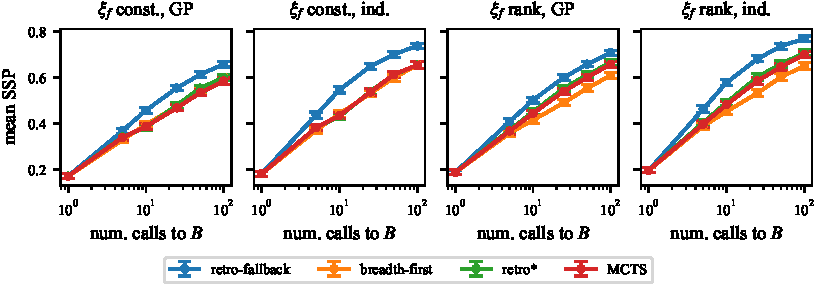
\includegraphics{figures/comparison/guacamol/ssp_sascore.pdf} \\
    \vspace{0.3cm}
    {\large optimistic heuristic} \\
    \vspace{0.3cm}
    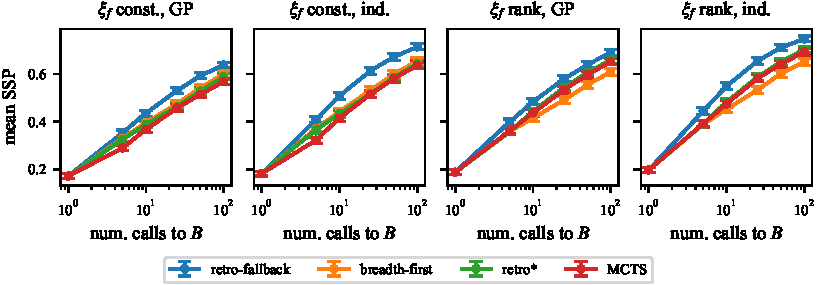
\includegraphics{figures/comparison/guacamol/ssp_optimistic.pdf}
    \caption[Mean SSP over time for GuacaMol molecules.]{
        Mean SSP vs time
        for 1000 molecules from GuacaMol.
        Interpretation is identical to 
        Figure~\ref{fig:ssp-rs190-sascore}.
    }
    \label{fig:ssp-guacamol-all-heuristics}
\end{figure}



A natural follow-up question is whether retro-fallback also performs well by metrics other than SSP.
In Figures~\ref{fig:most-feasible-route}--\ref{fig:fraction solved}
we plot the highest success probability of any \emph{individual} synthesis plan found,
plus two metrics frequently used by previous papers: the fraction of molecules with \emph{any} synthesis plan (called ``fraction solved'' in prior works) and
the length of the shortest synthesis plan found (a proxy for quality).
The SSP of the single best plan is generally similar for all algorithms.
This suggests that in general all algorithms find similar ``best'' plans,
and retro-fallback's extra success comes from finding more effective ``backup'' plans.
Retro-fallback seems slightly better than other algorithms in terms of fraction solved
and similar to other algorithms in terms of shortest plan length (although retro* is better in some cases).
Overall, these results suggest that retro-fallback is also an effective search algorithm if metrics from past papers which do not account for uncertainty are used.
\begin{figure}[htb]
    \centering
    {190 ``hard'' molecules; SA score heuristic} \\
    \vspace{0.3cm}
    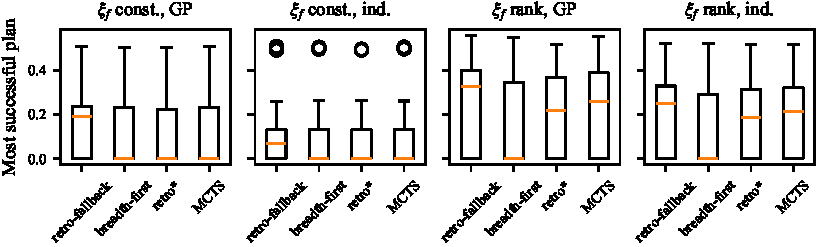
\includegraphics[width=0.8\textwidth]{figures/comparison/retrostar190/most_feasible_sascore.pdf} \\
    \vspace{0.3cm}
    {190 ``hard'' molecules; optimistic heuristic} \\
    \vspace{0.3cm}
    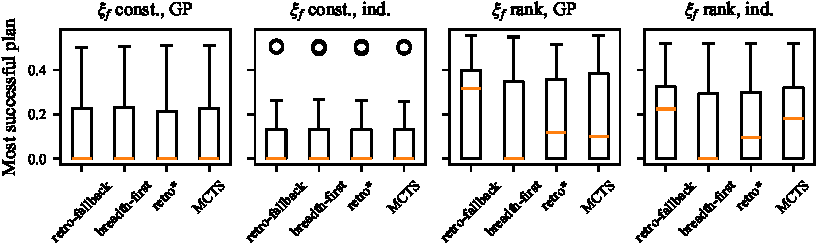
\includegraphics[width=0.8\textwidth]{figures/comparison/retrostar190/most_feasible_optimistic.pdf} \\
    \vspace{0.3cm}
    {GuacaMol; SA score heuristic} \\
    \vspace{0.3cm}
    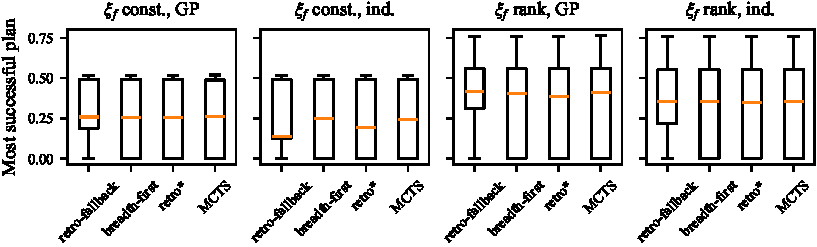
\includegraphics[width=0.8\textwidth]{figures/comparison/guacamol/most_feasible_sascore.pdf} \\
    \vspace{0.3cm}
    {GuacaMol; optimistic heuristic} \\
    \vspace{0.3cm}
    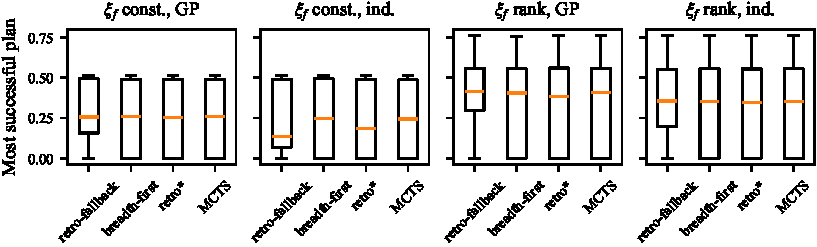
\includegraphics[width=0.8\textwidth]{figures/comparison/guacamol/most_feasible_optimistic.pdf}
    \caption[Success probability of most feasible synthesis plan.]{
        Success probability of most feasible synthesis plan
        at end of search
        (i.e.\@ $\max_{T\in\enumplans_{\targetmol}(\gG')}\sigma(T;\xi_f,\xi_b)$)
        for different algorithms.
    }
    \label{fig:most-feasible-route}
\end{figure}
\begin{figure}[htb]
    \centering
    {190 ``hard'' molecules; SA score heuristic} \\
    \vspace{0.3cm}
    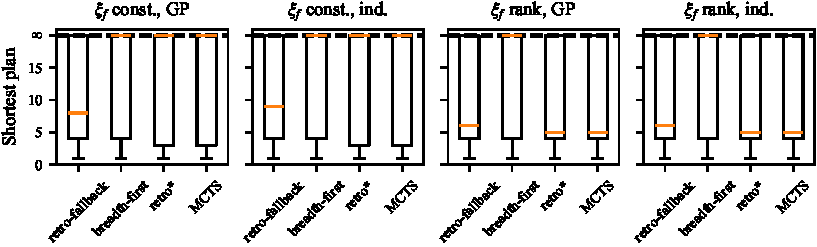
\includegraphics[width=0.8\textwidth]{figures/comparison/retrostar190/shortest_sascore.pdf} \\
    \vspace{0.3cm}
    {190 ``hard'' molecules; optimistic heuristic} \\
    \vspace{0.3cm}
    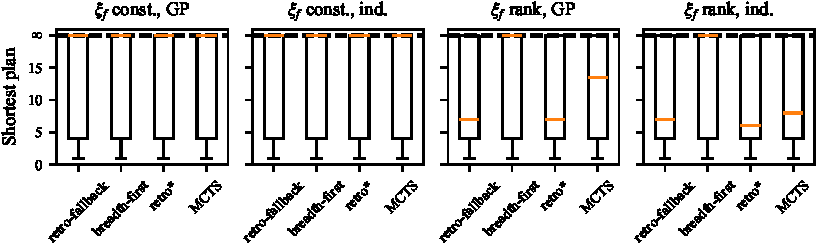
\includegraphics[width=0.8\textwidth]{figures/comparison/retrostar190/shortest_optimistic.pdf} \\
    \vspace{0.3cm}
    {GuacaMol; SA score heuristic} \\
    \vspace{0.3cm}
    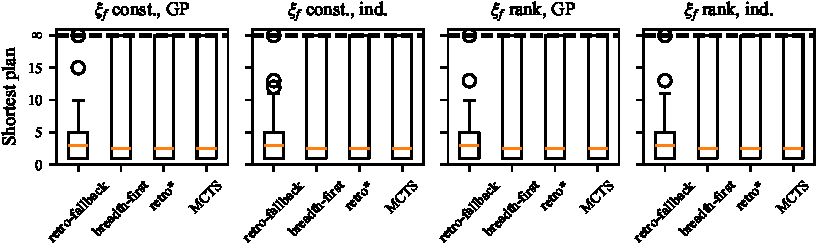
\includegraphics[width=0.8\textwidth]{figures/comparison/guacamol/shortest_sascore.pdf} \\
    \vspace{0.3cm}
    {GuacaMol; optimistic heuristic} \\
    \vspace{0.3cm}
    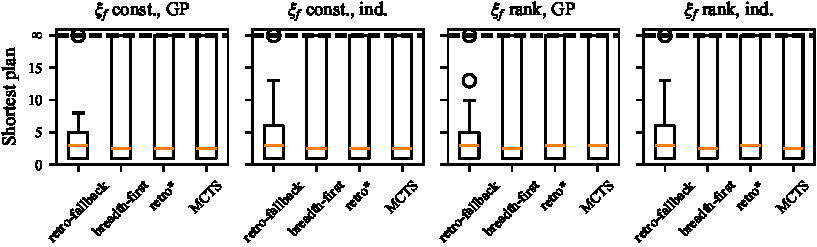
\includegraphics[width=0.8\textwidth]{figures/comparison/guacamol/shortest_optimistic.pdf}
    \caption[Length of shortest synthesis plan.]{
        Distribution of lengths of the shortest synthesis plan
        with non-zero success probability
        at end of search
        for different algorithms.
    }
    \label{fig:shortest-route}
\end{figure}
\begin{figure}[htb]
    \centering
    {190 ``hard'' molecules; SA score heuristic} \\
    \vspace{0.1cm}
    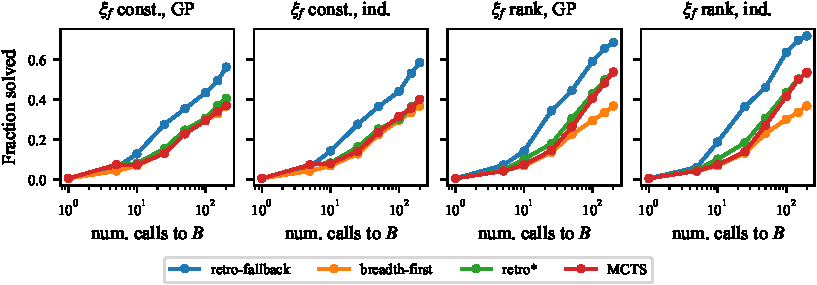
\includegraphics[width=0.8\textwidth]{figures/comparison/retrostar190/frac_solved_sascore.pdf} \\
    \vspace{0.1cm}
    {190 ``hard'' molecules; optimistic heuristic} \\
    \vspace{0.1cm}
    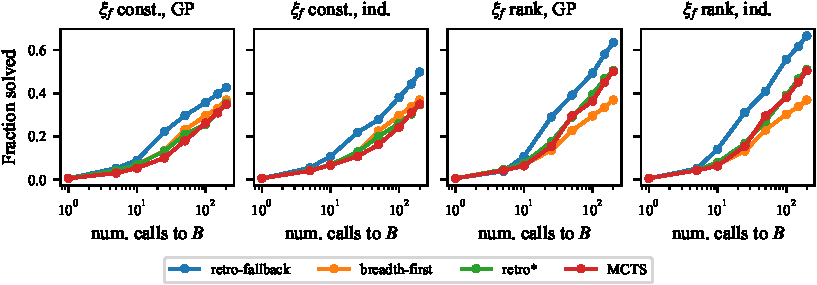
\includegraphics[width=0.8\textwidth]{figures/comparison/retrostar190/frac_solved_optimistic.pdf} \\
    \vspace{0.1cm}
    {GuacaMol; SA score heuristic} \\
    \vspace{0.1cm}
    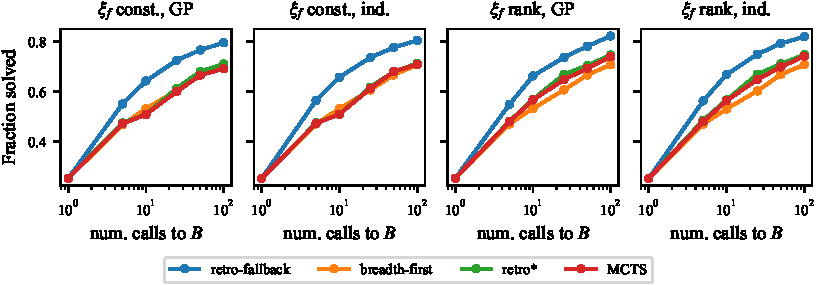
\includegraphics[width=0.8\textwidth]{figures/comparison/guacamol/frac_solved_sascore.pdf} \\
    \vspace{0.1cm}
    {GuacaMol; optimistic heuristic} \\
    \vspace{0.1cm}
    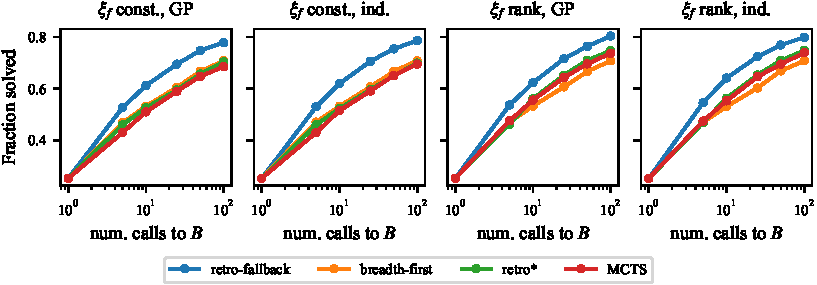
\includegraphics[width=0.8\textwidth]{figures/comparison/guacamol/frac_solved_optimistic.pdf}
    \caption[Fraction of molecules with any synthesis plan.]{
        Fraction of molecules for which a synthesis plan
        with non-zero success probability was found
        vs time
        for different algorithms.
    }
    \label{fig:fraction solved}
\end{figure}




\clearpage
\subsection{Speed and variability of retro-fallback}
\label{sec:experiment:speed and variability}

Next we consider the speed of retro-fallback.
Retro-fallback requires calculating $\rs$,
$\psi$, and $\rho$ for every node at every iteration.
The complexity of this calculation could scale linearly
with the number of nodes in the graph (which we denote $|\gG'|$),
or potentially sub-linearly if the $\rs$/$\psi$/$\rho$
values for many nodes do not change every iteration.
Therefore, from this step we would expect a time complexity
which is between linear and quadratic in $|\gG'|$.
However, retro-fallback also requires sampling $f$
and $b$ for all nodes created during an expansion:
a process which will scale as $\mathcal O(1)$
for independent models
and $\mathcal O (|\gG'|^2)$ for GP-correlated models.
This yields an overall  $\mathcal O (|\gG'|)$--$\mathcal O (|\gG'|^3)$
complexity from the sampling step.
Figure~\ref{fig:retro-fallback runtimes}
plots the empirical scaling for the experiments from the previous
section, and suggests an overall scaling between
$\mathcal O(|\gG'|^{1.1})$--$\mathcal O(|\gG'|^{1.8})$,
with considerable variation between different feasibility models
and heuristics.
\begin{figure}[ht]
    \centering
    {SA score heuristic} \\
    \vspace{0.3cm}
    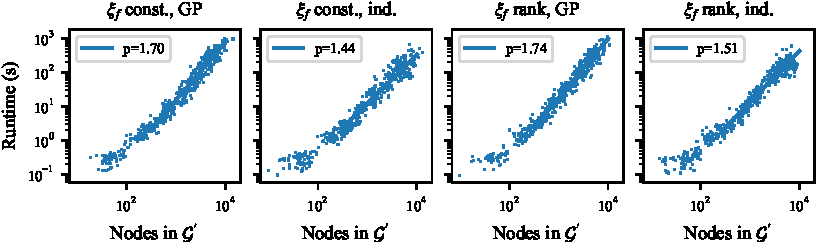
\includegraphics{figures/comparison/retrostar190/runtimes_sascore.pdf} \\
    \vspace{0.3cm}
    {optimistic heuristic} \\
    \vspace{0.3cm}
    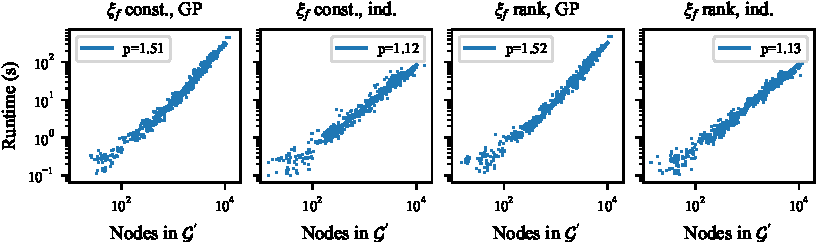
\includegraphics{figures/comparison/retrostar190/runtimes_optimistic.pdf}
    \caption[Time complexity of retro-fallback.]{
        Number of nodes vs total runtime
        for retro-fallback experiments
        on 190 ``hard'' molecule test set
        from section~\ref{sec:experiment:how effective is retro fallback},
        along with log-log fit of runtime 
        ($\log t=p\log{n} + C $).
    }
    \label{fig:retro-fallback runtimes}
\end{figure}

To study the effect of the number of samples $k$ from $\xi_f$ and $\xi_b$,
we run retro-fallback 10 times on a sub-sample of  25 molecules with a variety of different sample sizes.
Figure~\ref{fig:retro-fallback variability} shows that as $k$ decreases, the mean SSP value
achieved by retro-fallback
decreases and the variance of SSP increases.
This is not surprising, since when the number of samples is small
the internal estimates of SSP used by retro-fallback
deviate more from their expected values,
enabling suboptimal decisions.
Empirically, $k>100$ seems sufficient (minimal further improvement is seen for higher $k$).
\begin{figure}[ht]
    \centering
    {SA score heuristic} \\
    \vspace{0.3cm}
    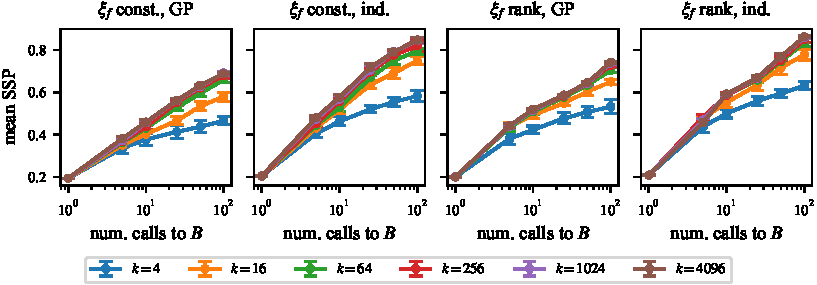
\includegraphics{figures/variation/guacamol/ssp_sascore.pdf} \\
    \vspace{0.3cm}
    {optimistic heuristic} \\
    \vspace{0.3cm}
    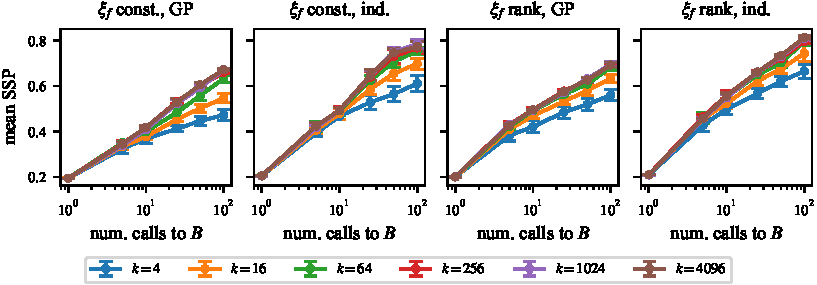
\includegraphics{figures/variation/guacamol/ssp_optimistic.pdf} \\
    \caption[Variation of retro-fallback with number of samples.]{
        Mean and standard deviation (over 10 trials)
        of average SSP for 25 molecules
        from the GuacaMol dataset
        when retro-fallback is run with different number
        of samples $k$
        for the feasibility and buyability models.
    }
    \label{fig:retro-fallback variability}
\end{figure}



\section{Discussion, Limitations, and Future Work}

In this chapter we reformulated retrosynthesis using stochastic processes,
presented a novel evaluation metric called ``successful synthesis probability'' (SSP),
and proposed a novel algorithm called retro-fallback which greedily maximises SSP.
In our experiments, retro-fallback was more effective at maximising SSP
than previously-proposed algorithms.

Our work has some important limitations.
Conceptually,
chemists may also care about the length or quality of synthesis plans,
and may only be willing to consider a limited number of backup plans.
Additionally, in practice the order of the steps in the synthesis plan is also important:
a synthesis plan whose first reaction is likely to fail is easy to try,
whereas a synthesis plan whose last reaction is likely to fail requires
investing time and resources into all previous steps before the feasibility of the last step can be tested.
Unfortunately, these considerations do not fit into our formalism,
which only considers whether or not a synthesis plan is executable.
It may be beneficial to modify retro-fallback to instead consider
the expected cost or number of steps required to complete a synthesis plan,
which would account for these other factors.
However, such a quantity may not be efficient to estimate like SSP,
creating the possibility that the resulting algorithm would not be tractable.
Investigating this could be an interesting direction for future work.

Moreover,
retro-fallback is slower than other algorithms and may not scale as well to larger search graphs.
It is unclear to what degree this can be improved.
Finally, the usefulness of the synthesis plans produced by retro-fallback
is clearly contingent on the quality of the feasibility and buyability models,
which at present are quite simple.

The most important direction for future work
is creating better models of reaction feasibility,
as without high-quality models the estimates of SSP are not meaningful.
We see collaborations with domain experts as the best route to achieve this.
Since retro-fallback uses a search heuristic,
learning this heuristic using the results of past searches (``self-play'')
would likely improve performance.
Overall, even though retro-fallback is far from perfect,
we believe that modelling uncertainty about reaction outcomes is at least
a step in the right direction,
and hope it inspires further work in this area.

\section{Retrospective and predictions}

Although this paper was published too recently to allow for a meaningful retrospective,
people with whom I have spoken about this work have all agreed with the motivation.
The main question asked is how to produce a good feasibility model,
which I believe is an important direction for future work.
